%Chapter 7

\chapter{On the Transferability of Deep-Q Networks} % Chapter title
\label{ch:dqn_transfer} % For referencing the chapter elsewhere, use \autoref{ch:introduction} 

\begin{remark}{Outline}
\end{remark}


\section{Motivation}





Model based transfer seems to work
No proper study in the model-free setting, no clear answer wrt transfer learning properties + limited set of algorithms and testing environments
Chapter before, extraordinarily long training times for benchmarks which are actually simple and sometimes not great performance neither -> tl could help achieve super human performance on environments which training from scratch appears to be limiting.


\section{A large-scale Empirical Study}
\label{sec:empirical_study}

We now present a large scale empirical study that investigates the transfer learning properties of convolutional neural networks that are trained for solving DRL tasks. Building on top of the research presented in the previous chapter, we keep considering model-free RL algorithms such as DQN, DDQN and DQV. We start by introducing the source and target Markov Decision Processes ($\mathcal{M}_S$, $\mathcal{M}_T$) used for our transfer learning study in Sec. \ref{sec:atari_environments}. We then present the adopted experimental setup in Sec. \ref{sec:experimental_setup_1}, where we describe our experiments and how we have quantitatively assessed the potential benefits of adopting transfer learning. We then report our results in Sec. \ref{sec:results_1} where we show that transferring pre-trained models in DRL is not as straightforward as it is in supervised learning. 


\subsection{The Atari Environments}
\label{sec:atari_environments}

As DRL testbed we keep using the Atari Arcade Learning Environment (ALE) that we have also adopted in the previous chapter when investigating the performance of DQV and DQV-Max Learning. Next to being one of the most popular benchmarks in DRL, the Atari suite provided by \citet{bellemare2013arcade} is particularly well suited for transfer learning research as it allows to choose among a set of $57$ Atari games that can be used as source and target MDPs within a deep transfer learning setting. Furthermore, despite each game coming with its own challenges, the way a state is represented and used as input for a convolutional neural network stays consistent across all Atari games, a property that makes it possible to use the same type of neural architecture over all $57$ environments, and that overcomes the need of having to define a new neural network for each game (which would make transfer learning impossible). Since training a DRL agent on the games of the ALE is a process which can go from lasting days to even weeks, we have carefully selected a subset of $10$ different environments that will serve for the transfer learning study presented in this chapter. These games are the following: . The game selection process was guided by numerous reasons. First, we have selected games for which we have the guarantee that a model-free DRL agent is able to learn a good policy for. Since, as discussed in Chapter \ref{ch:transfer_learning}, one of the key requirements of transfer learning is that of transferring knowledge across source and target tasks, we naturally ensured that some knowledge coming in the form of neural network parameters representing a near optimal value function was available for transfer. Second, while it is true that all of the selected games result in an agent that is able to improve its policy over time, some games were chosen because the learned policy resulted in a final performance that was not on par with that of a human expert player. This is for example the case of the \texttt{Frostbite} game, where the gap in performance between a DQV agent ($\approx 270$) and a human expert player ($\approx 4300$) is particularly significant. Therefore, it follows that \texttt{Frostbite} is a potentially interesting target task for transfer, as there is potentially room for improving the agent's performance through transfer learning. Furthermore, we have also ensured that among the selected games, some environments are more similar to each other than others. This if for example the case for the \texttt{Ms.Pacman} and \texttt{Bank Heist} games which, as can be seen in Fig. \ref{fig:similar_games}, are two games where the state space is represented as a maze, and where the end goal of an agent is that of learning how to navigate it. In like manner we have also included games which are very different from each other as is e.g., the case for the \texttt{Crazy Climber} and \texttt{Pong} games, where it is clear from Fig. \ref{fig:dissimilar_games} that no visual similarities are shared among the two environments. Including visually similar and dissimilar games easily allows us to investigate whether, as is the case in supervised learning, a source task is particularly well suited for transfer if it similar to its respective target task. 

\begin{figure}[ht]
\centering
\begin{minipage}[b]{0.45\linewidth}
\centering
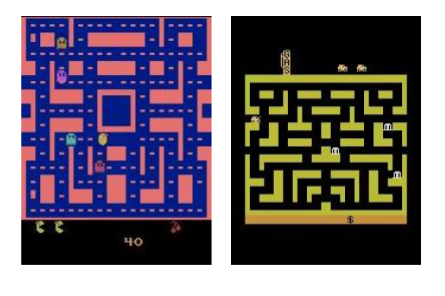
\includegraphics[width=\textwidth]{./Images/Chapter08/similar_sources}
\caption{The visually similar \texttt{Ms Pacman} and \texttt{Bank Heist} games.}
\label{fig:similar_games}
\end{minipage}
\hspace{0.5cm}
\begin{minipage}[b]{0.45\linewidth}
\centering
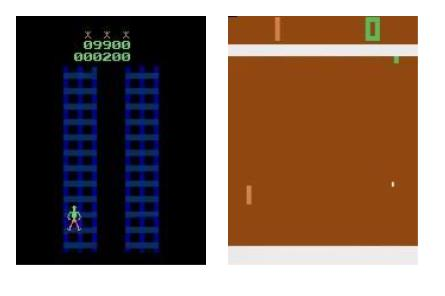
\includegraphics[width=\textwidth]{./Images/Chapter08/dissimilar_sources}
\caption{The highly different \texttt{Crazy Climber} and \texttt{Pong} games.}
\label{fig:dissimilar_games}
\end{minipage}
\end{figure}


\subsection{Experimental Setup}
\label{sec:experimental_setup_1}

Regarding the model-free DRL algorithms used for our study we investigate the transfer learning performance of agents that get trained with the DQV-Learning algorithm \cite{sabatelli2018deep} presented in Chapter \ref{ch:dqv_family_of_algorithms}, and with the DDQN algorithm \cite{van2016deep} reviewed in Chapter \ref{ch:reinforcement_learning}. We take models which come as pre-trained on the aforementioned Atari games and transfer them to all remaining environments. This is particularly easy to achieve as both algorithms learn an approximation of the optimal state-action value function $Q(s,a;\theta)$ by training a convolutional neural network directly on the images representing the state of the game. In fact, as mentioned beforehand, the state space across Atari games is always represented as a $84\times84\times4$ tensor, which makes it straightforward to transfer the same neural architecture among various Atari environments without needing special modifications. The only modification that we apply to a pre-trained network concerns its last layer responsible for estimating the different $Q$ values, which we always replace and randomly re-initialize. Following the typical deep transfer learning experimental setup discussed in Chapter \ref{ch:transfer_learning}, and motivated by the results obtained throughout the second part of this dissertation, we investigate whether in DRL it is as beneficial as it is in supervised learning to fine-tune a $\mathcal{M}_S$ pre-trained network on $\mathcal{M}_T$. We do this by quantitatively assessing the transfer learning benefits on each $\mathcal{M}_S/\mathcal{M}_T$ pair by computing the area ratio metric $r$ discussed by \citet{taylor2009transfer}. Specifically, given a learning curve representing the performance of an agent pre-trained on $\mathcal{M}_S$, and that of an agent that is instead trained from scratch, we compute $r$ as follows:
\begin{equation}
	r = \frac{\text{area of $\mathcal{M}_S$ $-$ area of $\mathcal{M}_T$}}{\text{area of $\mathcal{M}_T$}},
\label{eq:area_ratio_metric}
\end{equation}
where the area under the curve is approximated via trapezoidal numerical integration
\begin{equation}
	\int^{b}_{a}f(x)\:dx \approx(b-a) \cdot \frac{1}{2}(f(a)+f(b))
\end{equation}
and $a$ and $b$ correspond to the first and last training epochs respectively (see Fig. \ref{fig:area_under_curve} for a visualization of $r$).

\begin{figure}[ht!]
	\begin{tikzpicture}
\begin{axis}
[	grid style={dashed,gray},
	grid = both, 
	tick style=black,
  	xlabel=Epochs,
	ylabel = Reward,
]

\addlegendentry{DQV-Learning}

\addplot[blue, ultra thick] table[x=episodes,y=DQV] {./Results/Chapter07/logs/pong_results.txt};

\end{axis}
\end{tikzpicture}


\label{fig:area_under_curve}
\end{figure}

\subsection{Results}
\label{sec:results_1}

The results on each $\mathcal{M}_S/\mathcal{M}_T$ pair for the DQV and DDQN algorithms are presented in Tables \ref{tab:dqv_res} and \ref{tab:ddqn_res} respectively. In each cell of the tables we report the area ratio metric defined in Eq. \ref{eq:area_ratio_metric}, the lower this score, the redder the color of the cell, and therefore the less beneficial it is to transfer and fine-tune a pre-trained agent. When it comes to the DQV algorithm we can see that out of nine target environments, there is only one Atari game for which it is always beneficial to transfer and fine-tune a pre-trained model: \texttt{Fishing Derby}. In fact a positive area ratio score is obtained no matter which source environment is used for pre-training. It is worth noting however that the best results have been obtained when starting from an \texttt{Enduro} or \texttt{Pong} pre-trained network, which both resulted in an area ratio score of $\approx 0.72$. Positive transfer can also be observed on the \texttt{Frostbite} and \texttt{James Bond} games, although only for a very limited number of source games. For example, a \texttt{Bank Heist} pre-trained agent transfers well to both target games as it obtains an area ratio score of $0.729$ and $0.973$ respectively, whereas the same cannot be said for an \texttt{Enduro} pre-trained network which on \texttt{Frostbite} results in absent transfer (the area ratio score is in fact $-0.017$), and yields negative transfer on \texttt{James Bond} ($r=-0.41$). We can also observe that there are environments for which it is surprisingly never beneficial to transfer and fine-tune a pre-trained agent. This is for example the case for the \texttt{Bank Heist} and \texttt{Pong} games, where independently from which source game $\mathcal{M}_S$ is used for pre-training, a negative area ratio score is always obtained. Furthermore, it can also be observed that transfer learning across environments is not symmetric, as one source game $\mathcal{M}_S$ can result in positive transfer when it gets transferred to a certain target game $\mathcal{M}_T$ but the same outcome is not obtained when transfer is performed in the opposite direction. As an example we can consider the \texttt{Boxing/Fishing Derby} games: positive transfer is obtained when transferring from \texttt{Boxing}$\rightarrow$\texttt{Fishing Derby} ($r=0.552$), but negative transfer is obtained when transferring from \texttt{Fishing Derby} $\rightarrow$ \texttt{Boxing} ($r=-0.893$).  When it comes to the DDQN algorithm similar conclusions can be drawn: we can again observe that there are only very few cases for which it is beneficial to transfer and fine-tune a pre-trained DRL agent. Examples of such cases are networks that are pre-trained on \texttt{Ice Hockey} and \texttt{James Bond} which get transferred to \texttt{Boxing} ($r=0.245$ and $r=0.232$ respectively), or \texttt{Boxing} and \texttt{Enduro} models that get transferred to \texttt{Pong} ($r=0.936$ and $r=0.248$). \texttt{Bank Heist} and \texttt{Pong} are again the two target environments for which most of the transferred source models resulted in negative transfer, while we did not observe the positive transfer learning outcomes that characterized the DQV-Learning algorithm on \texttt{Fishing Derby}. Overall, fine-tuning a pre-trained DDQN agent mostly resulted in absent transfer as can especially be observed by the area ratio scores obtained on \texttt{Enduro, Fishing Derby, Gopher} and \texttt{Ice Hockey} which are $\approx 0$ on average.  

\begin{table}[ht!]
	\caption{The results obtained when fine-tuning ten different pre-trained DQV agents (rows) on nine other Atari games (columns). The lower the area ratio score, the redder the color of the cell. We can observe that fine-tuning a pre-trained agent is only beneficial on a limited set of target MDPs $\mathcal{M}_T$ such as \texttt{Fishing Derby}, where positive transfer is obtained no matter what source game is used for pre-training, and \texttt{James Bond}, where negative transfer is only obtained when using \texttt{Enduro} and \texttt{Zaxxon} as source games.}
	\newcommand*{\MinNumber}{-1}%
\newcommand*{\MaxNumber}{1}%

\newcommand{\ApplyGradient}[1]{%
  \pgfmathsetmacro{\PercentColor}{100.0*(#1-\MaxNumber)/(\MinNumber-\MaxNumber)}%
  %\textcolor{black!\PercentColor}{#1}
  \edef\x{\noexpand\cellcolor{red!\PercentColor}}\x\textcolor{black}{#1}%
}
\newcolumntype{R}{>{\collectcell\ApplyGradient}{c}<{\endcollectcell}}

\resizebox{\columnwidth}{!}{%
\begin{tabular}{c|R|R|R|R|R|R|R|R|R|R}
\hline 
{} & BankHeist & Boxing & CrazyClimber & Enduro & FishingDerby & Frostbite & JamesBond & MsPacman &   Pong & Zaxxon \\
\hline \hline 
BankHeist    &     -      & -0.019 &           -1 & -0.317 &          0.5 &     0.729 &     0.973 &   -0.089 & -1.238 & -0.998 \\
Boxing       &    -0.494 &    -    &       -0.278 & -0.852 &        0.552 &     -0.01 &     0.247 &   -0.184 & -0.841 & -0.999 \\
CrazyClimber &    -0.569 & -0.261 &           -   & -0.593 &         0.19 &     0.277 &     0.621 &   -0.111 & -1.206 & -0.178 \\
Enduro       &    -0.571 & -0.018 &        -0.25 &     -   &        0.726 &    -0.017 &     -0.41 &    -0.08 & -0.466 & -0.164 \\
FishingDerby &        -1 & -0.893 &       -0.093 &  -0.45 &            -  &     0.068 &     0.197 &   -0.136 & -3.083 & -0.999 \\
Frostbite    &    -0.933 &  0.024 &           -1 & -0.348 &        0.222 &        -   &     0.569 &    0.009 & -0.663 & -0.076 \\
JamesBond    &    -0.123 & -0.106 &       -0.131 & -0.033 &        0.519 &     0.262 &         -  &    0.218 & -1.329 &     -1 \\
MsPacman     &    -0.985 & -0.219 &       -0.012 & -0.494 &          0.6 &     0.346 &     0.398 &        -  & -1.646 & -0.997 \\
Pong         &        -1 & -0.083 &       -0.428 & -0.476 &        0.725 &    -0.024 &     0.896 &    0.123 &    -    & -0.729 \\
Zaxxon       &     -0.76 & -0.028 &        0.037 & -0.116 &        0.385 &      0.16 &    -0.253 &     0.06 & -1.602 &   -     \\
\end{tabular}%
}


	\label{tab:dqv_res}
\end{table}


\begin{table}[ht!]
	\caption{The results obtained when fine-tuning ten different pre-trained DDQN agents (rows) on nine other Atari games (columns). Similarly to Table \ref{tab:dqv_res} the lower the area ratio score, the redder the color of the cell. We can again observe that fine-tuning a pre-trained agent is only beneficial in a very limited number of cases and that the DDQN algorithm results in different transfer learning performance than DQV.}
	\newcommand*{\MinNumber}{-1}%
\newcommand*{\MaxNumber}{1}%

\newcommand{\ApplyGradient}[1]{%
  \pgfmathsetmacro{\PercentColor}{100.0*(#1-\MaxNumber)/(\MinNumber-\MaxNumber)}%
  %\textcolor{black!\PercentColor}{#1}
  \edef\x{\noexpand\cellcolor{red!\PercentColor}}\x\textcolor{black}{#1}%
}
\newcolumntype{R}{>{\collectcell\ApplyGradient}{c}<{\endcollectcell}}

\resizebox{\columnwidth}{!}{%
\begin{tabular}{c|R|R|R|R|R|R|R|R|R|R}
\hline 
{} & BankHeist & Boxing & CrazyClimber & Enduro & FishingDerby & Gopher & IceHockey & Jamesbond & MsPacman & Pong \\
\hline\hline
BankHeist    &       -                    &                  0.121 &                       -0.378 &                 -0.006 &                       -0.107 &                  0.042 &                    -0.006 &                    -0.058 &                    0.001 &               -3.013 \\
Boxing       &                    -0.316 &     -                   &                       -0.104 &                     -0 &                        0.038 &                   0.06 &                     0.015 &                    -0.225 &                   -0.027 &                0.936 \\
CrazyClimber &                    -0.192 &                 -0.487 &               -               &                 -0.012 &                       -0.084 &                  0.016 &                     0.015 &                     0.016 &                   -0.015 &                -2.64 \\
Enduro       &                    -0.296 &                  0.193 &                       -0.167 &       -                 &                        0.039 &                   0.03 &                     0.019 &                    -0.235 &                   -0.039 &                0.248 \\
FishingDerby &                    -0.212 &                 -0.545 &                           -1 &                 -0.085 &         -                     &                  0.016 &                     0.001 &                    -0.055 &                   -0.026 &               -0.935 \\
Gopher       &                    -0.466 &                  0.044 &                       -0.108 &                 -0.005 &                        0.007 &            -            &                    -0.005 &                    -0.094 &                    -0.02 &               -1.816 \\
IceHockey    &                    -0.046 &                  0.245 &                       -0.067 &                  0.014 &                       -0.178 &                  0.072 &            -               &                     0.037 &                   -0.015 &                0.112 \\
Jamesbond    &                    -0.145 &                  0.232 &                       -0.064 &                  0.005 &                       -0.267 &                  0.031 &                    -0.092 &      -                     &                   -0.006 &               -1.578 \\
MsPacman     &                    -0.173 &                 -1.179 &                       -0.129 &                  -0.06 &                        0.003 &                 -0.019 &                     0.007 &                     0.071 &       -                   &               -2.774 \\
Pong         &                    -0.127 &                  0.028 &                        -0.12 &                   0.01 &                        0.037 &                  0.042 &                     0.002 &                    -0.174 &                   -0.006 &             -         \\
\end{tabular}%
}

	\label{tab:ddqn_res}
\end{table}


\section{Control Experiments}

The results presented in the previous section seem to be questioning the level of transferability of convolutional neural networks that get trained for solving RL tasks. In fact, the training strategy of fine-tuning a pre-trained model on $\mathcal{M}_T$ does not result in the same type of performance gains that we have extensively observed throughout the second part of this dissertation, when pre-trained models were transferred and fine-tuned in a supervised learning context. To better characterize the transfer learning properties of pre-trained convolutional neural networks for DRL, we have designed a set of simple control experiments that allow us to examine their transfer learning behavior in training conditions that are as similar as possible to the ones of the experimental setup adopted in Sec. \ref{sec:empirical_study}. The main difference, however, is that the RL tasks that will be considered from now on, are much simpler than the ones defined within the ALE environment, and therefore do not require extraordinarily long training times for learning an optimal policy.   

\subsection{The Catch Environments}
\label{sec:catch_environments}

To this end we have implemented four different versions of the \texttt{Catch} game, a simple RL task that was first presented by \citet{mnih2014recurrent}, and that has been widely used within the literature for investigating the performance of DRL algorithms in a fast, and computationally less expensive manner than the one usually required by the \tattt{Atari} games \cite{vanjos2018deep, aittahar2020empirical}. In the game of \texttt{Catch}, an agent controls a paddle at the bottom of the environment, represented by a $21 \times 21$ grid, and has to catch a ball falling from top to bottom which can potentially bounce off walls. At each time-step, the agent can choose between three different actions: move the paddle one pixel to the right, move it to the left, or do not perform any of the aforementioned actions, therefore keeping its paddle in the same position in the grid. A RL episode ends either when the agent manages to catch the ball, in which case it receives a reward of $1$, or when it misses the ball, which naturally results in a reward of $0$. Following the design choices presented in \cite{vanjos2017deep}, we model the ball to have vertical speed of $v_y=-1 \: cell/s$ and horizontal speed of $v_x \in \{-2,-1,0,1,2\}$. From now on we will refer to this version of the game as \texttt{Catch-v0}, as it is the most basic and simplest form of the game that will be used throughout our experiments (see Fig. \ref{fig:fig1} for an impression of the game). Next to \texttt{Catch-v0} we have implemented three, slightly different and arguably more complex versions of the game as well. The first of such versions is \texttt{Catch-v1}, visually represented in Fig. \ref{fig:fig2}, where the complexity of the game is increased by reducing the size of the paddle that is controlled by the agent. While for \texttt{Catch-v0} its size is of five pixels, in \texttt{Catch-v1} it is of two pixels, therefore requiring the agent to be more precise if it wants to successfully catch the falling ball. The second alternative version of \texttt{Catch} is \texttt{Catch-v2}. In this case, the dynamics of the game are identical to the ones that define \texttt{Catch-v0}, however, as can be seen in Fig. \ref{fig:fig3} the way the $21 \times 21$ grid is represented changes. While in \texttt{Catch-v0} as well as in \texttt{Catch-v1} the state is represented by a binary grid where all pixels, but the ones representing the paddle and the ball have a value of $0$, in \texttt{Catch-v3} the cells around the paddle and the ball can have a random value between $0$ and $255$. This design choice makes it much harder for a convolutional network to correctly locate and identify the position of the paddle and of the falling ball, and makes \texttt{Catch-v2} the arguably most complex version among the different \texttt{Catch} versions of the game. Lastly we have implemented \texttt{Catch-v3}, a version of \texttt{Catch} which is identical to the one that is modeled by \texttt{Catch-v0} with the main difference that the representation of the state is now mirrored (see Fig. \ref{fig:fig4}), therefore requiring the agent to look at different parts of the grid if it wants to locate the paddle, and understand that the ball is unnaturally moving from the bottom to the top.  

\begin{figure}[ht]
\centering
\begin{minipage}[b]{0.35\linewidth}
\centering
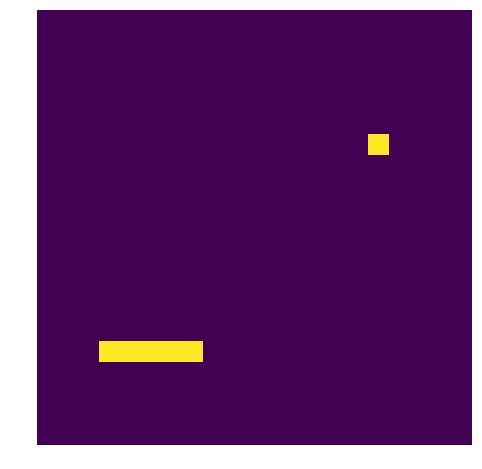
\includegraphics[width=\textwidth]{./Images/Chapter08/catch_v0}
\caption{\texttt{Catch-v0}}
\label{fig:fig1}
\end{minipage}
\hspace{0.5cm}
\begin{minipage}[b]{0.35\linewidth}
\centering
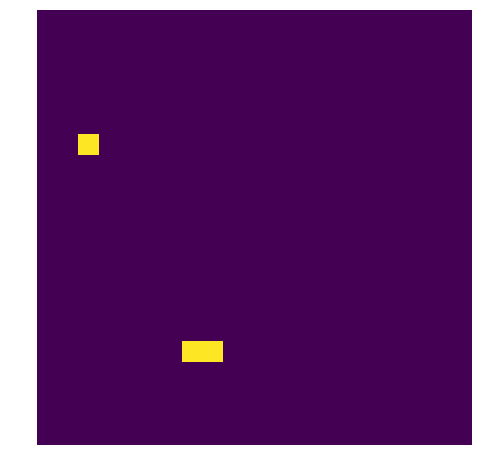
\includegraphics[width=\textwidth]{./Images/Chapter08/catch_v2}
\caption{\texttt{Catch-v1}}
\label{fig:fig2}
\end{minipage}
\hspace{0.5cm}
\begin{minipage}[b]{0.35\linewidth}
\centering
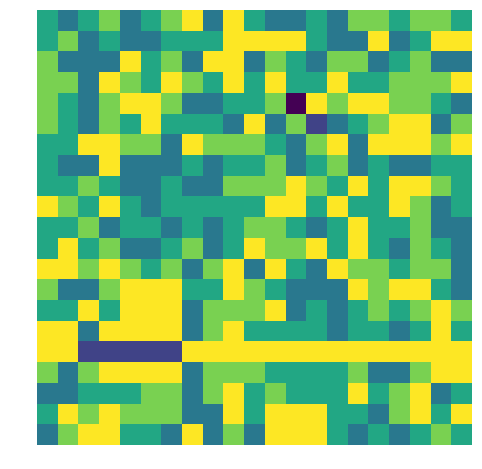
\includegraphics[width=\textwidth]{./Images/Chapter08/catch_v3}
\caption{\texttt{Catch-v2}}
\label{fig:fig3}
\end{minipage}
\hspace{0.5cm}
\begin{minipage}[b]{0.35\linewidth}
\centering
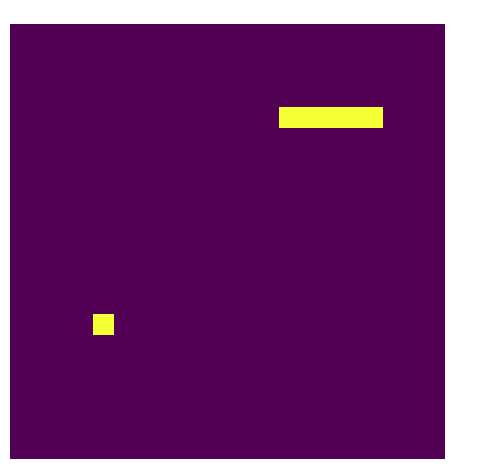
\includegraphics[width=\textwidth]{./Images/Chapter08/catch_v1}
\caption{\texttt{Catch-v3}}
\label{fig:fig4}
\end{minipage}
\end{figure}


\paragraph{Experimental Setup}
\label{sec:experimental_setup_control}
Given the overall simplicity of the different \texttt{Catch} environments, we now train a DQN agent instead of the arguably more complex DQV and DDQN agents that we considered in Sec. \ref{sec:empirical_study}. The agent comes in the form a two-hidden layer convolutional neural network which is followed by a fully connected layer of $256$ hidden units preceding the final linear layer responsible for estimating the different $Q(s,a)$ values. The first convolutional layer has $32$ channels whereas the second one has $64$ channels. All layers of the network are activated by a ReLU non-linearity. We use an experience replay memory buffer that is set to contain $400000$ trajectories, and start training the model as soon as $5000$ trajectories have been collected. For exploration purposes, we adopt the popular epsilon-greedy strategy with an initial $\epsilon$ value of $1$ which gets linearly annealed over time to $0.1$. Learning a near optimal policy on the aforementioned \texttt{Catch} environments with this type of DQN agent can require between the $3$ and the $5$ hours of training time. We visualize the learning curves for each of the four different \texttt{Catch} environments in Fig. \ref{fig:catch_baselines}, where for every training epoch (reported on the $x$ axis) we report the average performance that is obtained by an agent that is evaluated on ten different episodes ($y$ axis). Shaded areas around the line plots correspond to $\pm 1$ std. deviation obtained over five different training runs with five different random seeds.    

\paragraph{DQN Performance}
As we can see from the results reported in Fig. \ref{fig:catch_baselines}, the DQN agent described above is able to successfully learn a near optimal policy for all \texttt{Catch} versions. When it comes to \texttt{Catch-v0}, \texttt{Catch-v2} and \texttt{Catch-v3} we can observe that by the end of training the agent is able to catch $\approx 100\%$ of the falling balls, whereas its performance is slightly worse ($\approx 90\%$) when it comes to \texttt{Catch-v1} \footnote{Please note that the performance on \texttt{Catch-v1} can be improved by increasing the complexity of the DQN agent by adding one more convolutional layer. However, as the goal is to transfer the same type of model across \texttt{Catch} games we did not modify the architecture of the DQN agent, at the cost of having a slightly worse performing model.}. We can also observe that among the different \texttt{Catch} versions, \texttt{Catch-v0} and \texttt{Catch-v3} appear to be the easiest ones, as the agent requires significantly less training episodes to converge when compared to \texttt{Catch-v1} and \texttt{Catch-v2}. Furthermore, in line with the explanation presented beforehand, our results also confirm the hypothesis that \texttt{Catch-v2} is the overall most complicated \texttt{Catch} version, as learning requires significantly more, and potentially unstable, training epochs.

\begin{figure}
\centering
\begin{tikzpicture}
\begin{axis}
[	grid style={dashed,gray},
	grid = both, 
	tick style=black,
  	xlabel=Epochs,
	ylabel = $\%$ of caught balls,
	legend style={at={(-0.3,-0.3,-0.4)},anchor=south west,legend columns=4},
]

\addlegendentry{\texttt{Catch-v0}}

\addplot[blue, ultra thick] table[x=epochs,y=catchv0] {./Results/Chapter08/logs/catch_baselines.dat};
\addplot[name path=upper,draw=none, forget plot] table[x=epochs,y expr=\thisrow{catchv0}+\thisrow{stdv0}] {./Results/Chapter08/logs/catch_baselines.dat};
\addplot[name path=lower,draw=none, forget plot] table[x=epochs,y expr=\thisrow{catchv0}-\thisrow{stdv0}] {./Results/Chapter08/logs/catch_baselines.dat};
\addplot[fill=blue!10, forget plot] fill between[of=upper and lower];

\addlegendentry{\texttt{Catch-v1}}
\addplot[ultra thick, yellow] table[x=epochs,y=catchv3] {./Results/Chapter08/logs/catch_baselines.dat};
\addplot [name path=upper,draw=none, forget plot] table[x=epochs,y expr=\thisrow{catchv3}+\thisrow{stdv3}] {./Results/Chapter08/logs/catch_baselines.dat};
\addplot [name path=lower,draw=none, forget plot] table[x=epochs,y expr=\thisrow{catchv3}-\thisrow{stdv3}] {./Results/Chapter08/logs/catch_baselines.dat};
\addplot [fill=yellow!10, forget plot] fill between[of=upper and lower];

\addlegendentry{\texttt{Catch-v2}}
\addplot[ultra thick, red] table[x=epochs,y=catchv1] {./Results/Chapter08/logs/catch_baselines.dat};
\addplot[name path=upper,draw=none, forget plot] table[x=epochs,y expr=\thisrow{catchv1}+\thisrow{stdv1}] {./Results/Chapter08/logs/catch_baselines.dat};
\addplot[name path=lower,draw=none, forget plot] table[x=epochs,y expr=\thisrow{catchv1}-\thisrow{stdv1}] {./Results/Chapter08/logs/catch_baselines.dat};
\addplot[fill=red!10, forget plot] fill between[of=upper and lower];

\addlegendentry{\texttt{Catch-v3}}
\addplot[ultra thick, green] table[x=epochs,y=catchv2] {./Results/Chapter08/logs/catch_baselines.dat};
\addplot [name path=upper,draw=none, forget plot] table[x=epochs,y expr=\thisrow{catchv2}+\thisrow{stdv2}] {./Results/Chapter08/logs/catch_baselines.dat};
\addplot [name path=lower,draw=none, forget plot] table[x=epochs,y expr=\thisrow{catchv2}-\thisrow{stdv2}] {./Results/Chapter08/logs/catch_baselines.dat};
\addplot [fill=green!10, forget plot] fill between[of=upper and lower];

\end{axis}
\end{tikzpicture}


\caption{Learning curves obtained by a DQN agent that is trained from scratch on the four different versions of the \texttt{Catch} game presented in Sec. \ref{sec:catch_environments}. We can see that \texttt{Catch-v0} and \texttt{Catch-v3} are equivalent in terms of complexity as they require the $\approx$ same number of training episodes to to reach convergence, whereas \textttt{Catch-v1} and \texttt{Catch-v2} result in an agent that either obtains on average lower rewards (\texttt{Catch-v1}), or converges slower (\texttt{Catch-v2}).}
\label{fig:catch_baselines}
\end{figure}

\subsection{From one Catch to Another}
\label{sec:from_one_catch_to_another}

We now replicate the TL study presented in Sec. \ref{sec:empirical_study} on the aforementioned \texttt{Catch} environments, with the hope of identifying why the process of fine-tuning a pre-trained convolutional neural network in a DRL context, seems to not be as beneficial as it is in the supervised learning one. To this end, our goal is to find at least one pair of \texttt{Catch} environments which results in positive transfer, and to then potentially identify some properties within the different \texttt{Catch} versions that could also hold for the pairs of \texttt{Atari} games which have yielded positive transfer in Tables \ref{tab:dqv_res} and \ref{tab:ddqn_res}. Specifically, we formulate \textcolor{RoyalBlue}{two hypothesis}, based on which, we expect to experimentally observe positive transfer. First, we foresee that positive transfer will happen for all possible \texttt{Catch} combinations, as in the end the source MDP $\mathcal{M}_S$ and the target MDP $\mathcal{M}_T$ do not significantly differ from each other: in fact, the main task across the different \texttt{Catch} versions remains that of catching a falling ball; the action space is identical; and so is the reward function that always returns a value of $1$ when the agent succeeds in catching the falling ball. This hypothesis is also motivated by the results that we presented throughout the first part of this dissertation, where we showed that the higher the similarity between the source domain $\mathcal{D}_S$ and the target domain $\mathcal{D}_T$, the better the performance of a transferred pre-trained network. Second, in the case the previous hypothesis will not be empirically supported, we expect to at least observe positive transfer when using a model that comes as pre-trained either on \texttt{Catch-v1} or on \texttt{Catch-v2}. In fact, as described above and also shown by the performance reported in Fig. \ref{fig:catch_baselines}, these variants of the game can be considered as the two most complicated versions of the \texttt{Catch} environment. This hypothesis is motivated by numerous claims that stem from transfer learning research performed in computer vision. Indeed, when it comes to supervised learning, one of the main factors that makes a certain source task $\mathcal{T}_S$ good for transferring is its complexity \cite{mensink2021factors}, which is usually defined in terms of dataset size and number of classes to classify. We therefore expect the complexity of the source MDP $\mathcal{M}_S$ to play an important role within DRL as well. Similarly to what we did for DQV and DDQN in Sec. \ref{sec:empirical_study}, we take the four different models that have been trained from scratch on their respective \texttt{Catch} version, randomly re-initialize their last layer (responsible for estimating the different state-action values $Q(s,a)$) and fully fine-tune the pre-trained network on the three remaining \texttt{Catch} environments, following the experimental protocol described in Sec. \ref{sec:experimental_setup_control}. The results of this study are reported in Fig. \ref{fig:catch_transfer}, where in clockwise order we show the performance that is obtained when considering \texttt{Catch-v0}, \texttt{Catch-v1}, \texttt{Catch-v2} and \texttt{Catch-v3} as target MDP $\mathcal{M}_T$. The performance of each transferred network is compared against the performance that is obtained after training a DQN agent from scratch which matches with the results reported in Fig. \ref{fig:catch_baselines}.
Surprisingly we found that fine-tuning a pre-trained DQN agent never resulted in positive transfer learning. This can clearly be seen in all plots represented in Fig. \ref{fig:catch_transfer} and by the results reporting the area ratio metric in Table \ref{tab:catch_tl_area_ratio}. The only case where starting from a pre-trained network appeared to be at least in part beneficial is represented by the first plot of Fig. \ref{fig:catch_transfer} when \texttt{Catch-v1} is considered as source MDP $\mathcal{M}_S$. In this case we can in fact observe some learning speed improvements within the first $25$ learning epochs. This is not surprising as an agent which is able to catch a ball with a small paddle (as defined by the game \texttt{Catch-v1}) should in principle also be able to do this when the size of its paddle is larger (which is the case for \texttt{Catch-v0}). What is more surprising, however, is that while training progresses we see that the performance of a \texttt{Catch-v1} pre-trained model starts deteriorating and that this model barely converges to the same performance that is obtained by a model trained from scratch. When it comes to all other $\mathcal{M}_S-\mathcal{M}_T$ pairs we see that pre-trained networks always perform significantly worse than randomly initialized models trained from scratch, with some extreme cases, as the ones reported for the pair represented in the last plot of Fig. \ref{fig:catch_transfer}, where a pre-trained agent is barely able to improve its policy over time at all. These results invalidate our two hypotheses mentioned above as they clearly show that positive transfer in DRL does not arise when $\mathcal{M}_S$ and $\mathcal{M}_T$ are similar, nor when $\mathcal{M}_S$ is more complex than $\mathcal{M}_T$. 

\begin{figure}[ht!]
\resizebox{0.45\textwidth}{!}{  \centering
\begin{tikzpicture}
\begin{axis}
[	
	name=ax1,	
	grid style={dashed,gray},
	grid = both, 
	tick style=black,
  	xlabel=Epochs,
	ylabel = $\%$ of caught balls,
	title = \texttt{Catch-v0},
	legend pos=south east,	
]


%\addlegendentry{\texttt{Catch-v0}}
\addplot[blue, ultra thick] table[x=epochs,y=target_catch] {./Results/Chapter08/logs/catch_v0.dat};
\addplot [name path=upper,draw=none, forget plot] table[x=epochs,y expr=\thisrow{target_catch}+\thisrow{std_target_catch}] {./Results/Chapter08/logs/catch_v0.dat};
\addplot [name path=lower,draw=none, forget plot] table[x=epochs,y expr=\thisrow{target_catch}-\thisrow{std_target_catch}] {./Results/Chapter08/logs/catch_v0.dat};
\addplot [fill=blue!10, forget plot] fill between[of=upper and lower];

%\addlegendentry{\texttt{Catch-v1}}
\addplot[ultra thick, red] table[x=epochs,y=Catch_v2] {./Results/Chapter08/logs/catch_v0.dat};
\addplot [name path=upper,draw=none, forget plot] table[x=epochs,y expr=\thisrow{Catch_v2}+\thisrow{Catch_v2_std}] {./Results/Chapter08/logs/catch_v0.dat};
\addplot [name path=lower,draw=none, forget plot] table[x=epochs,y expr=\thisrow{Catch_v2}-\thisrow{Catch_v2_std}] {./Results/Chapter08/logs/catch_v0.dat};
\addplot [fill=red!10, forget plot] fill between[of=upper and lower];

%\addlegendentry{\texttt{Catch-v2}}
\addplot[ultra thick, green] table[x=epochs,y=Catch_v3] {./Results/Chapter08/logs/catch_v0.dat};
\addplot [name path=upper,draw=none, forget plot] table[x=epochs,y expr=\thisrow{Catch_v3}+\thisrow{Catch_v3_std}] {./Results/Chapter08/logs/catch_v0.dat};
\addplot [name path=lower,draw=none, forget plot] table[x=epochs,y expr=\thisrow{Catch_v3}-\thisrow{Catch_v3_std}] {./Results/Chapter08/logs/catch_v0.dat};
\addplot [fill=green!10, forget plot] fill between[of=upper and lower];

%\addlegendentry{\texttt{Catch-v3}}
\addplot[ultra thick, yellow] table[x=epochs,y=Catch_v4] {./Results/Chapter08/logs/catch_v0.dat};
\addplot [name path=upper,draw=none, forget plot] table[x=epochs,y expr=\thisrow{Catch_v4}+\thisrow{Catch_v4_std}] {./Results/Chapter08/logs/catch_v0.dat};
\addplot [name path=lower,draw=none, forget plot] table[x=epochs,y expr=\thisrow{Catch_v4}-\thisrow{Catch_v4_std}] {./Results/Chapter08/logs/catch_v0.dat};
\addplot [fill=yellow!10, forget plot] fill between[of=upper and lower];

\end{axis}


\begin{axis}
[	
	at={(ax1.south east)},
	xshift=1cm,
	grid style={dashed,gray},
	grid = both, 
	tick style=black,
  	xlabel=Epochs,
	%ylabel = $\%$ of caught balls,
	title = \texttt{Catch-v1},
	legend pos=south east,
]

%\addlegendentry{\texttt{Catch-v0}}

\addplot[yellow, ultra thick] table[x=epochs,y=target_catch] {./Results/Chapter08/logs/catch_v1.dat};
\addplot [name path=upper,draw=none, forget plot] table[x=epochs,y expr=\thisrow{target_catch}+\thisrow{std_target_catch}] {./Results/Chapter08/logs/catch_v1.dat};
\addplot [name path=lower,draw=none, forget plot] table[x=epochs,y expr=\thisrow{target_catch}-\thisrow{std_target_catch}] {./Results/Chapter08/logs/catch_v1.dat};
\addplot [fill=yellow!10, forget plot] fill between[of=upper and lower];

%\addlegendentry{\texttt{Catch-v2}}
\addplot[ultra thick, red] table[x=epochs,y=Catch_v0] {./Results/Chapter08/logs/catch_v1.dat};
\addplot [name path=upper,draw=none, forget plot] table[x=epochs,y expr=\thisrow{Catch_v0}+\thisrow{Catch_v0_std}] {./Results/Chapter08/logs/catch_v1.dat};
\addplot [name path=lower,draw=none, forget plot] table[x=epochs,y expr=\thisrow{Catch_v0}-\thisrow{Catch_v0_std}] {./Results/Chapter08/logs/catch_v1.dat};
\addplot [fill=red!10, forget plot] fill between[of=upper and lower];

%\addlegendentry{\texttt{Catch-v1}}
\addplot[ultra thick, green] table[x=epochs,y=Catch_v2] {./Results/Chapter08/logs/catch_v1.dat};
\addplot [name path=upper,draw=none, forget plot] table[x=epochs,y expr=\thisrow{Catch_v2}+\thisrow{Catch_v2_std}] {./Results/Chapter08/logs/catch_v1.dat};
\addplot [name path=lower,draw=none, forget plot] table[x=epochs,y expr=\thisrow{Catch_v2}-\thisrow{Catch_v2_std}] {./Results/Chapter08/logs/catch_v1.dat};
\addplot [fill=green!10, forget plot] fill between[of=upper and lower];

%\addlegendentry{\texttt{Catch-v3}}
\addplot[ultra thick, blue] table[x=epochs,y=Catch_v3] {./Results/Chapter08/logs/catch_v1.dat};
\addplot [name path=upper,draw=none, forget plot] table[x=epochs,y expr=\thisrow{Catch_v3}+\thisrow{Catch_v3_std}] {./Results/Chapter08/logs/catch_v1.dat};
\addplot [name path=lower,draw=none, forget plot] table[x=epochs,y expr=\thisrow{Catch_v3}-\thisrow{Catch_v3_std}] {./Results/Chapter08/logs/catch_v1.dat};
\addplot [fill=blue!10, forget plot] fill between[of=upper and lower];

\end{axis}


\begin{axis}
[	at={(ax1.south east)},
	xshift=9cm,
    grid style={dashed,gray},
	grid = both, 
	tick style=black,
  	xlabel=Epochs,
	%ylabel = $\%$ of caught balls,
	legend pos=south east,	
	title = \texttt{Catch-v2}
]


%\addlegendentry{\texttt{Catch-v0}}
\addplot[red, ultra thick] table[x=epochs,y=target_catch] {./Results/Chapter08/logs/catch_v2.dat};
\addplot [name path=upper,draw=none, forget plot] table[x=epochs,y expr=\thisrow{target_catch}+\thisrow{std_target_catch}] {./Results/Chapter08/logs/catch_v2.dat};
\addplot [name path=lower,draw=none, forget plot] table[x=epochs,y expr=\thisrow{target_catch}-\thisrow{std_target_catch}] {./Results/Chapter08/logs/catch_v2.dat};
\addplot [fill=red!10, forget plot] fill between[of=upper and lower];

%\addlegendentry{\texttt{Catch-v1}}
\addplot[ultra thick, blue] table[x=epochs,y=Catch_v0] {./Results/Chapter08/logs/catch_v2.dat};
\addplot [name path=upper,draw=none, forget plot] table[x=epochs,y expr=\thisrow{Catch_v0}+\thisrow{Catch_v0_std}] {./Results/Chapter08/logs/catch_v2.dat};
\addplot [name path=lower,draw=none, forget plot] table[x=epochs,y expr=\thisrow{Catch_v0}-\thisrow{Catch_v0_std}] {./Results/Chapter08/logs/catch_v2.dat};
\addplot [fill=blue!10, forget plot] fill between[of=upper and lower];

%\addlegendentry{\texttt{Catch-v2}}
\addplot[ultra thick, green] table[x=epochs,y=Catch_v3] {./Results/Chapter08/logs/catch_v2.dat};
\addplot [name path=upper,draw=none, forget plot] table[x=epochs,y expr=\thisrow{Catch_v3}+\thisrow{Catch_v3_std}] {./Results/Chapter08/logs/catch_v2.dat};
\addplot [name path=lower,draw=none, forget plot] table[x=epochs,y expr=\thisrow{Catch_v3}-\thisrow{Catch_v3_std}] {./Results/Chapter08/logs/catch_v2.dat};
\addplot [fill=green!10, forget plot] fill between[of=upper and lower];

%\addlegendentry{\texttt{Catch-v3}}
\addplot[ultra thick, yellow] table[x=epochs,y=Catch_v4] {./Results/Chapter08/logs/catch_v2.dat};
\addplot [name path=upper,draw=none, forget plot] table[x=epochs,y expr=\thisrow{Catch_v4}+\thisrow{Catch_v4_std}] {./Results/Chapter08/logs/catch_v2.dat};
\addplot [name path=lower,draw=none, forget plot] table[x=epochs,y expr=\thisrow{Catch_v4}-\thisrow{Catch_v4_std}] {./Results/Chapter08/logs/catch_v2.dat};
\addplot [fill=yellow!10, forget plot] fill between[of=upper and lower];

\end{axis}


\begin{axis}
[	
    at={(ax1.south east)},
	xshift=17cm,
    grid style={dashed,gray},
	grid = both, 
	tick style=black,
  	xlabel=Epochs,
	%ylabel = $\%$ of caught balls,
	%legend style={at={(-1,-0.4,-1.4)},anchor=south,legend columns=4},
	title= \texttt{Catch-v3}
]

\addlegendentry{\texttt{Catch-v0}}
\addplot[ultra thick, blue] table[x=epochs,y=Catch_v0] {./Results/Chapter08/logs/catch_v3.dat};
\addplot [name path=upper,draw=none, forget plot] table[x=epochs,y expr=\thisrow{Catch_v0}+\thisrow{Catch_v0_std}] {./Results/Chapter08/logs/catch_v3.dat};
\addplot [name path=lower,draw=none, forget plot] table[x=epochs,y expr=\thisrow{Catch_v0}-\thisrow{Catch_v0_std}] {./Results/Chapter08/logs/catch_v3.dat};
\addplot [fill=blue!10, forget plot] fill between[of=upper and lower];


\addlegendentry{\texttt{Catch-v1}}
\addplot[ultra thick, yellow] table[x=epochs,y=Catch_v4] {./Results/Chapter08/logs/catch_v3.dat};
\addplot [name path=upper,draw=none, forget plot] table[x=epochs,y expr=\thisrow{Catch_v4}+\thisrow{Catch_v4_std}] {./Results/Chapter08/logs/catch_v3.dat};
\addplot [name path=lower,draw=none, forget plot] table[x=epochs,y expr=\thisrow{Catch_v4}-\thisrow{Catch_v4_std}] {./Results/Chapter08/logs/catch_v3.dat};
\addplot [fill=yellow!10, forget plot] fill between[of=upper and lower];

\addlegendentry{\texttt{Catch-v2}}
\addplot[ultra thick, red] table[x=epochs,y=Catch_v2] {./Results/Chapter08/logs/catch_v3.dat};
\addplot [name path=upper,draw=none, forget plot] table[x=epochs,y expr=\thisrow{Catch_v2}+\thisrow{Catch_v2_std}] {./Results/Chapter08/logs/catch_v3.dat};
\addplot [name path=lower,draw=none, forget plot] table[x=epochs,y expr=\thisrow{Catch_v2}-\thisrow{Catch_v2_std}] {./Results/Chapter08/logs/catch_v3.dat};
\addplot [fill=red!10, forget plot] fill between[of=upper and lower];


\addlegendentry{\texttt{Catch-v3}}
\addplot[green, ultra thick] table[x=epochs,y=target_catch] {./Results/Chapter08/logs/catch_v3.dat};
\addplot [name path=upper,draw=none, forget plot] table[x=epochs,y expr=\thisrow{target_catch}+\thisrow{std_target_catch}] {./Results/Chapter08/logs/catch_v3.dat};
\addplot [name path=lower,draw=none, forget plot] table[x=epochs,y expr=\thisrow{target_catch}-\thisrow{std_target_catch}] {./Results/Chapter08/logs/catch_v3.dat};
\addplot [fill=green!10, forget plot] fill between[of=upper and lower];



\end{axis}


\end{tikzpicture}%
}
\caption{The results obtained after using a pre-trained \texttt{Catch} agent and fine-tuning it on a different \texttt{Catch} version. We can observe that despite all \texttt{Catch} versions being very similar no positive transfer is ever observed, as a model trained from scratch always outperforms a pre-trained, fine-tuned network.}
\label{fig:catch_transfer}
\end{figure}


\begin{table}
	\centering
	\caption{The area ratio obtained after fine-tuning a pre-trained DQN agent on the different \texttt{Catch} environments. We can see that no matter which source game is used for pre-training, transfer learning surprisingly always results in negative transfer.}
	\newcommand*{\MinNumber}{-0.479}%
\newcommand*{\MaxNumber}{0.1}%

\newcommand{\ApplyGradient}[1]{%
  \pgfmathsetmacro{\PercentColor}{100.0*(#1-\MaxNumber)/(\MinNumber-\MaxNumber)}%
  %\textcolor{black!\PercentColor}{#1}
  \edef\x{\noexpand\cellcolor{red!\PercentColor}}\x\textcolor{black}{#1}%
}
\newcolumntype{R}{>{\collectcell\ApplyGradient}{c}<{\endcollectcell}}
\begin{tabular}{c|R|R|R|R}
\hline 
{} & Catch-v0 & Catch-v2 & Catch-v3 & Catch-v4 \\ \hline\hline
Catch-v0 &       -   &   -0.026 &   -0.486 &   -0.479 \\
Catch-v2 &    -0.16 &       -   &   -0.121 &   -0.248 \\
Catch-v3 &   -0.406 &   -0.313 &      -    &   -0.465 \\
Catch-v4 &   -0.016 &    -0.24 &   -0.179 &       -   \\
\end{tabular}

	\label{tab:catch_tl_area_ratio}
\end{table}


\subsection{Self-Transfer}
\label{sec:self_transfer}

The surprisingly poor transfer learning performance observed in the previous experiment made us question the level of transferability of Deep-Q Networks even more. To further characterize their TL properties we decided to investigate whether pre-trained DRL agents are at least able to transfer to themselves. To this end we studied what happens when a DQN agent gets transferred to a version of \texttt{Catch} that matches with the version of the game that was also used during the pre-training stage. This experiment is in large part identical to the one presented in Sec. \ref{sec:from_one_catch_to_another}, with the only difference being that now $\mathcal{M}_S = \mathcal{M}_T$. Moreover, differently from the previous study, we now also investigate what happens if instead of fine-tuning the network completely we just use the pre-trained DQN agent as a simple feature extractor, therefore only training its last layer responsible for estimating the different state-action values. Our results are presented in Fig. \ref{fig:catch_self_transfer}, where for each \texttt{Catch} version the full lines represent the performance of a network that is trained from scratch, whereas the dashed and dotted lines respectively report the performance that is obtained when the network is either used as simple feature extractor or entirely fine-tuned. We can see that if a pre-trained Deep-Q Network is used as a simple feature extractor, then the agent is able to converge to the optimal policy almost immediately. In fact as can consistently be observed in all plots of Fig. \ref{fig:catch_self_transfer} and from the results presented in Table \ref{tab:self_tl_area_ratio}, training only the last layer of a pre-trained network yields positive transfer for all different \texttt{Catch} versions. However, when a fine-tuning training strategy is adopted much more surprising results have been obtained. First, and more importantly, we can see that despite all models showing some learning speed improvements at early training iterations, their final performance is never on par with the one that is obtained when the same kind of model is either used as a feature extractor or trained from scratch (the dotted lines are consistently below the dashed and full lines). While when it comes to \texttt{Catch-v0} the policy learned by a fine-tuned model still allows the agent to successfully catch $\approx 95\%$ of the falling balls, the same cannot be said when the models are tested on \texttt{Catch-v1, Catch-v2} and \texttt{Catch-v3}, where the difference in terms of performance between a model trained from scratch and a fine-tuned one is much more significant. Please also note that special attention should be given to \texttt{Catch-v2}, which is an environment where the area ratio score reported in Table \ref{tab:self_tl_area_ratio} can be misleading as it does not entirely reflect the quality of the final policy learned by the agent. In fact, while it is true that an $r$ value of $0.393$ is obtained, it is worth noting that a fine-tuned network converges to a policy which is significantly worse than the one of a network trained from scratch, as the agent that is only able of catching $\approx 80\%$ of the falling balls. Second, as highlighted by the large variance across different training runs, fine-tuning on \texttt{Catch-v1} and \texttt{Catch-v3} resulted in highly unstable learning as well.    

\begin{figure}[ht]
  \centering
 \resizebox{\columnwidth}{!}{%
\begin{tikzpicture}
\begin{axis}
[	
	name=ax1,	
	grid style={dashed,gray},
	grid = both, 
	tick style=black,
  	xlabel=Epochs,
	ylabel = $\%$ of caught balls,
	title = \texttt{Catch-v0},
	legend pos=south east,	
]

\addlegendentry{\texttt{Catch-v0}}
\addplot[blue, ultra thick] table[x=epochs,y=baseline] {./Results/Chapter08/logs/self_transfer_catch_v0.dat};
\addplot [name path=upper,draw=none] table[x=epochs,y expr=\thisrow{baseline}+\thisrow{std_baseline}] {./Results/Chapter08/logs/self_transfer_catch_v0.dat};
\addplot [name path=lower,draw=none] table[x=epochs,y expr=\thisrow{baseline}-\thisrow{std_baseline}] {./Results/Chapter08/logs/self_transfer_catch_v0.dat};
\addplot [fill=blue!10] fill between[of=upper and lower];

\addlegendentry{\texttt{Only Head}}
\addplot[ultra thick, red] table[x=epochs,y=only_head] {./Results/Chapter08/logs/self_transfer_catch_v0.dat};
\addplot [name path=upper,draw=none] table[x=epochs,y expr=\thisrow{only_head}+\thisrow{std_only_head}] {./Results/Chapter08/logs/self_transfer_catch_v0.dat};
\addplot [name path=lower,draw=none] table[x=epochs,y expr=\thisrow{only_head}-\thisrow{std_only_head}] {./Results/Chapter08/logs/self_transfer_catch_v0.dat};
\addplot [fill=red!10] fill between[of=upper and lower];

\addlegendentry{\texttt{Full Fine-Tuning}}
\addplot[ultra thick, green] table[x=epochs,y=self_transfer_full_fine_tuning] {./Results/Chapter08/logs/self_transfer_catch_v0.dat};
\addplot [name path=upper,draw=none] table[x=epochs,y expr=\thisrow{self_transfer_full_fine_tuning}+\thisrow{std_self_transfer_full_fine_tuning}] {./Results/Chapter08/logs/self_transfer_catch_v0.dat};
\addplot [name path=lower,draw=none] table[x=epochs,y expr=\thisrow{self_transfer_full_fine_tuning}-\thisrow{std_self_transfer_full_fine_tuning}] {./Results/Chapter08/logs/self_transfer_catch_v0.dat};
\addplot [fill=green!10] fill between[of=upper and lower];

\end{axis}


\begin{axis}
[	
	at={(ax1.south east)},
	xshift=2cm,	
	grid style={dashed,gray},
	grid = both, 
	tick style=black,
  	xlabel=Epochs,
	ylabel = $\%$ of caught balls,
	title = \texttt{Catch-v0},
	legend pos=south east,	
]

\addlegendentry{\texttt{Catch-v0}}
\addplot[blue, ultra thick] table[x=epochs,y=baseline] {./Results/Chapter08/logs/self_transfer_catch_v1.dat};
\addplot [name path=upper,draw=none] table[x=epochs,y expr=\thisrow{baseline}+\thisrow{std_baseline}] {./Results/Chapter08/logs/self_transfer_catch_v1.dat};
\addplot [name path=lower,draw=none] table[x=epochs,y expr=\thisrow{baseline}-\thisrow{std_baseline}] {./Results/Chapter08/logs/self_transfer_catch_v1.dat};
\addplot [fill=blue!10] fill between[of=upper and lower];

\addlegendentry{\texttt{Only Head}}
\addplot[ultra thick, red] table[x=epochs,y=only_head] {./Results/Chapter08/logs/self_transfer_catch_v1.dat};
\addplot [name path=upper,draw=none] table[x=epochs,y expr=\thisrow{only_head}+\thisrow{std_only_head}] {./Results/Chapter08/logs/self_transfer_catch_v1.dat};
\addplot [name path=lower,draw=none] table[x=epochs,y expr=\thisrow{only_head}-\thisrow{std_only_head}] {./Results/Chapter08/logs/self_transfer_catch_v1.dat};
\addplot [fill=red!10] fill between[of=upper and lower];

\addlegendentry{\texttt{Full Fine-Tuning}}
\addplot[ultra thick, green] table[x=epochs,y=self_transfer_full_fine_tuning] {./Results/Chapter08/logs/self_transfer_catch_v1.dat};
\addplot [name path=upper,draw=none] table[x=epochs,y expr=\thisrow{self_transfer_full_fine_tuning}+\thisrow{std_self_transfer_full_fine_tuning}] {./Results/Chapter08/logs/self_transfer_catch_v1.dat};
\addplot [name path=lower,draw=none] table[x=epochs,y expr=\thisrow{self_transfer_full_fine_tuning}-\thisrow{std_self_transfer_full_fine_tuning}] {./Results/Chapter08/logs/self_transfer_catch_v1.dat};
\addplot [fill=green!10] fill between[of=upper and lower];

\end{axis}


\end{tikzpicture}%
}

 \resizebox{\columnwidth}{!}{%
\begin{tikzpicture}
\begin{axis}
[	
	name=ax1,	
	grid style={dashed,gray},
	grid = both, 
	tick style=black,
  	xlabel=Epochs,
	ylabel = $\%$ of caught balls,
	title = \texttt{Catch-v0},
	legend pos=south east,	
]

\addlegendentry{\texttt{Catch-v0}}
\addplot[blue, ultra thick] table[x=epochs,y=baseline] {./Results/Chapter08/logs/self_transfer_catch_v2.dat};
\addplot [name path=upper,draw=none] table[x=epochs,y expr=\thisrow{baseline}+\thisrow{std_baseline}] {./Results/Chapter08/logs/self_transfer_catch_v2.dat};
\addplot [name path=lower,draw=none] table[x=epochs,y expr=\thisrow{baseline}-\thisrow{std_baseline}] {./Results/Chapter08/logs/self_transfer_catch_v2.dat};
\addplot [fill=blue!10] fill between[of=upper and lower];

\addlegendentry{\texttt{Only Head}}
\addplot[ultra thick, red] table[x=epochs,y=only_head] {./Results/Chapter08/logs/self_transfer_catch_v2.dat};
\addplot [name path=upper,draw=none] table[x=epochs,y expr=\thisrow{only_head}+\thisrow{std_only_head}] {./Results/Chapter08/logs/self_transfer_catch_v2.dat};
\addplot [name path=lower,draw=none] table[x=epochs,y expr=\thisrow{only_head}-\thisrow{std_only_head}] {./Results/Chapter08/logs/self_transfer_catch_v2.dat};
\addplot [fill=red!10] fill between[of=upper and lower];

\addlegendentry{\texttt{Full Fine-Tuning}}
\addplot[ultra thick, green] table[x=epochs,y=self_transfer_full_fine_tuning] {./Results/Chapter08/logs/self_transfer_catch_v2.dat};
\addplot [name path=upper,draw=none] table[x=epochs,y expr=\thisrow{self_transfer_full_fine_tuning}+\thisrow{std_self_transfer_full_fine_tuning}] {./Results/Chapter08/logs/self_transfer_catch_v2.dat};
\addplot [name path=lower,draw=none] table[x=epochs,y expr=\thisrow{self_transfer_full_fine_tuning}-\thisrow{std_self_transfer_full_fine_tuning}] {./Results/Chapter08/logs/self_transfer_catch_v2.dat};
\addplot [fill=green!10] fill between[of=upper and lower];

\end{axis}


\begin{axis}
[	
	at={(ax1.south east)},
	xshift=2cm,	
	grid style={dashed,gray},
	grid = both, 
	tick style=black,
  	xlabel=Epochs,
	ylabel = $\%$ of caught balls,
	title = \texttt{Catch-v0},
	legend pos=south east,	
]

\addlegendentry{\texttt{Catch-v0}}
\addplot[blue, ultra thick] table[x=epochs,y=baseline] {./Results/Chapter08/logs/self_transfer_catch_v3.dat};
\addplot [name path=upper,draw=none] table[x=epochs,y expr=\thisrow{baseline}+\thisrow{std_baseline}] {./Results/Chapter08/logs/self_transfer_catch_v3.dat};
\addplot [name path=lower,draw=none] table[x=epochs,y expr=\thisrow{baseline}-\thisrow{std_baseline}] {./Results/Chapter08/logs/self_transfer_catch_v3.dat};
\addplot [fill=blue!10] fill between[of=upper and lower];

\addlegendentry{\texttt{Only Head}}
\addplot[ultra thick, red] table[x=epochs,y=only_head] {./Results/Chapter08/logs/self_transfer_catch_v3.dat};
\addplot [name path=upper,draw=none] table[x=epochs,y expr=\thisrow{only_head}+\thisrow{std_only_head}] {./Results/Chapter08/logs/self_transfer_catch_v3.dat};
\addplot [name path=lower,draw=none] table[x=epochs,y expr=\thisrow{only_head}-\thisrow{std_only_head}] {./Results/Chapter08/logs/self_transfer_catch_v3.dat};
\addplot [fill=red!10] fill between[of=upper and lower];

\addlegendentry{\texttt{Full Fine-Tuning}}
\addplot[ultra thick, green] table[x=epochs,y=self_transfer_full_fine_tuning] {./Results/Chapter08/logs/self_transfer_catch_v3.dat};
\addplot [name path=upper,draw=none] table[x=epochs,y expr=\thisrow{self_transfer_full_fine_tuning}+\thisrow{std_self_transfer_full_fine_tuning}] {./Results/Chapter08/logs/self_transfer_catch_v3.dat};
\addplot [name path=lower,draw=none] table[x=epochs,y expr=\thisrow{self_transfer_full_fine_tuning}-\thisrow{std_self_transfer_full_fine_tuning}] {./Results/Chapter08/logs/self_transfer_catch_v3.dat};
\addplot [fill=green!10] fill between[of=upper and lower];

\end{axis}


\end{tikzpicture}%
}
\caption{hello}
\label{fig:catch_self_transfer}
\end{figure}


\begin{table}
	\centering
	\caption{The area ratio scores obtained after performing self-transfer. We can see that if only the last linear layer is trained, then positive transfer is obtained on all \texttt{Catch} environments, whereas if the network is fine-tuned, positive transfer is (in part) only obtained on \texttt{Catch-v2}.}
	\newcommand*{\MinNumber}{-0.236}%
\newcommand*{\MaxNumber}{0.674}%

\newcommand{\ApplyGradient}[1]{%
  \pgfmathsetmacro{\PercentColor}{100.0*(#1-\MaxNumber)/(\MinNumber-\MaxNumber)}%
  %\textcolor{black!\PercentColor}{#1}
  \edef\x{\noexpand\cellcolor{red!\PercentColor}}\x\textcolor{black}{#1}%
}
\newcolumntype{R}{>{\collectcell\ApplyGradient}{c}<{\endcollectcell}}
\begin{tabular}{c|R|R|R|R}
\hline 
           &  Catch-v0 & Catch-v1 & Catch-v2 & Catch-v3 \\ \hline \hline
Only-Head   & 0.05     & 0.141    & 0.674    & 0.059    \\
Fine-Tuning & 0.017    & -0.218   & 0.393    & -0.236   \\   
\end{tabular}	

	\label{tab:self_tl_area_ratio}
\end{table}

\section{The Two Training Phases of Deep-Q Networks}
\label{sec:hybrid_self_transfer}

To investigate the hypothesis that convolutional neural networks ... we have designed the following experiment. Let us start by visually representing the pre-trained convolutional neural networks that we have trained in Sec. \ref{sec:self_transfer}. Recall that when performing a self-transfer experiment we always start with a model that is pre-trained on a source task that is identical to the target task. As is common within DRL, this kind of model corresponds to a network that estimates as many $Q(s,a)$ values as there are actions available to an agent. This is done after having performed a series of convolutions that are usually followed by a fully connected layer (see Sec. \ref{sec:experimental_setup_control} for additional details). It follows that when training a prototypical Q-Network, a DRL agent goes through two very distinctive phases: a feature extraction phase, and a phase which is responsible for estimating the optimal $Q$ values. We visually represent such a model in the first image of Fig. \ref{fig:networks}, where the parts of the network that are involved in the feature extraction phase are colored in green, while the final linear layer responsible for modeling $Q(s,a)$ is colored in red. Following the experimental protocol and the results presented in Sec. \ref{sec:self_transfer}, we know that such a model results in positive transfer when its last linear layer is trained after being randomly re-initialized, whereas it yields negative transfer if a fine-tuning training strategy is adopted. These two transfer learning approaches are represented in the second and third images of Fig. \ref{fig:networks}. Note in fact, that when the last layer is trained, we only change the color of the final output nodes from red to purple (see second image), whereas the colors of the entire network are changed to yellow and blue if the network is fine-tuned.  

\begin{figure}[ht!]
\centering
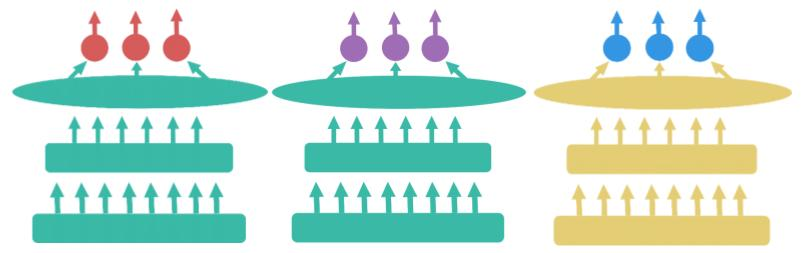
\includegraphics[width=\textwidth]{./Images/Chapter08/networks.jpg}
\caption{Three visual representations of the convolutional neural networks whose performance is reported in Fig. \ref{fig:catch_self_transfer}. In the first plot a network that simply comes as pre-trained on a certain source-task. In the second plot the same model which only updates the weights that are responsible for modeling the $Q$ function. In the third plot, a pre-trained model which gets wholly fine-tuned and therefore, once transferred, updates all of its parameters.}
\label{fig:networks}
\end{figure}

With these concepts in place, we are ready to describe our final self-transfer experiment. We investigate the transfer learning performance of a model that is a combination between the one depicted in the second image of Fig. \ref{fig:networks}, and the one represented in the third image of Fig. \ref{fig:networks}. Specifically, we fine-tune a neural network whose last linear layer is initialized with the parameters that yielded positive transfer in Sec. \ref{sec:self_transfer}, whereas its convolutional and fully connected layers are initialized with the parameters that yielded negative transfer, which therefore correspond to weights that are the result of wholly fine-tuning a pre-trained model. The resulting architecture is visually represented in Fig. \ref{fig:hybrid_network}.

\begin{figure}[ht!]
\centering
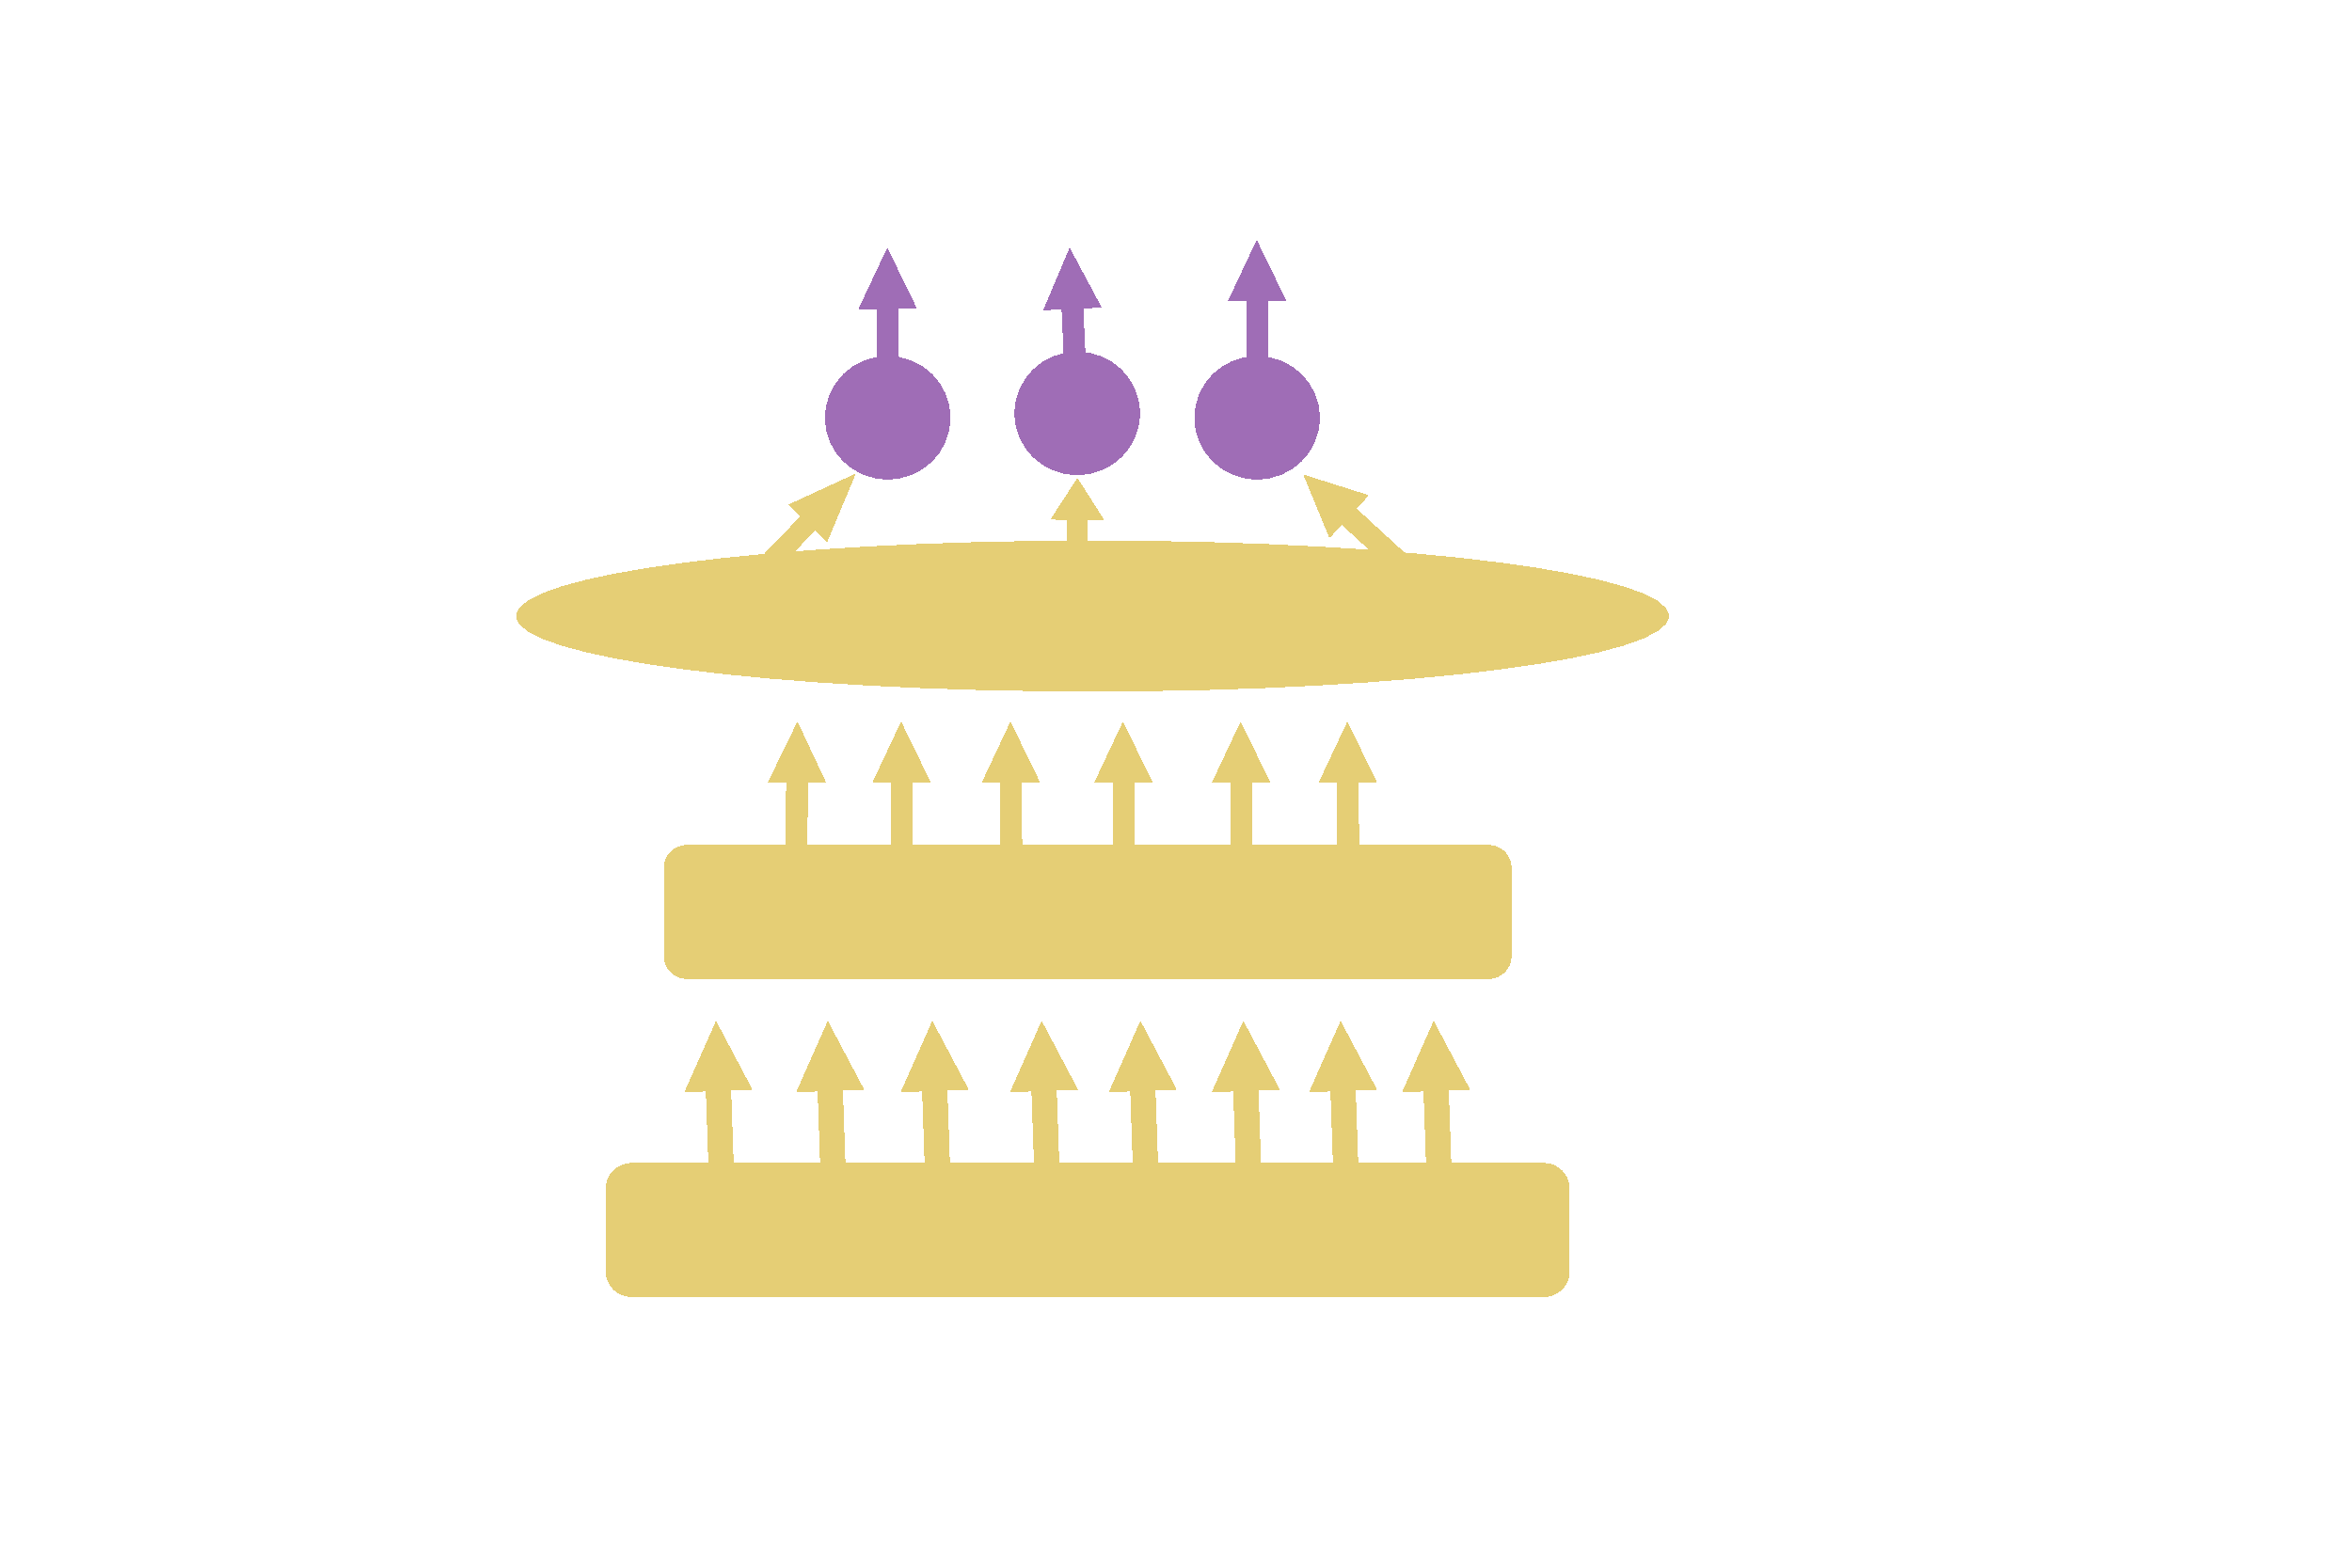
\includegraphics[width=\textwidth]{./Images/Chapter08/hybrid_network.pdf}
\caption{A pre-trained Deep-Q Network whose convolutional and fully connected layers are initialized with weights that resulted in negative transfer, while its final linear layer is instead initialized with weights that resulted in positive transfer.}
\label{fig:hybrid_network}
\end{figure}


\subsection{Results}
\begin{figure}[ht!]
  \centering

\resizebox{\columnwidth}{!}{%
\begin{tikzpicture}
\begin{axis}
[	
	name=ax1,	
	grid style={dashed,gray},
	grid = both, 
	tick style=black,
  	xlabel=Epochs,
	ylabel = $\%$ of caught balls,
	title = \texttt{Catch-v0},
	legend pos=south east,	
]

\addlegendentry{\texttt{Catch-v0}}
\addplot[blue, ultra thick] table[x=epochs,y=baseline] {./Results/Chapter08/logs/hybrid_self_tl_v0.dat};
\addplot [name path=upper,draw=none] table[x=epochs,y expr=\thisrow{baseline}+\thisrow{std_baseline}] {./Results/Chapter08/logs/hybrid_self_tl_v0.dat};
\addplot [name path=lower,draw=none] table[x=epochs,y expr=\thisrow{baseline}-\thisrow{std_baseline}] {./Results/Chapter08/logs/hybrid_self_tl_v0.dat};
\addplot [fill=blue!10] fill between[of=upper and lower];


\addlegendentry{\texttt{Full Fine-Tuning}}
\addplot[dashed, ultra thick,blue] table[x=epochs,y=self_transfer_full_fine_tuning] {./Results/Chapter08/logs/hybrid_self_tl_v0.dat};
\addplot [name path=upper,draw=none] table[x=epochs,y expr=\thisrow{self_transfer_full_fine_tuning}+\thisrow{std_self_transfer_full_fine_tuning}] {./Results/Chapter08/logs/hybrid_self_tl_v0.dat};
\addplot [name path=lower,draw=none] table[x=epochs,y expr=\thisrow{self_transfer_full_fine_tuning}-\thisrow{std_self_transfer_full_fine_tuning}] {./Results/Chapter08/logs/hybrid_self_tl_v0.dat};
\addplot [fill=blue!10] fill between[of=upper and lower];

\addlegendentry{\texttt{Hybrid Fine-Tuning}}
\addplot[dashed, ultra thick,gray] table[x=epochs,y=hybrid_self_transfer] {./Results/Chapter08/logs/hybrid_self_tl_v0.dat};
\addplot [name path=upper,draw=none] table[x=epochs,y expr=\thisrow{hybrid_self_transfer}+\thisrow{std_hybrid_self_transfer}] {./Results/Chapter08/logs/hybrid_self_tl_v0.dat};
\addplot [name path=lower,draw=none] table[x=epochs,y expr=\thisrow{hybrid_self_transfer}-\thisrow{std_hybrid_self_transfer}] {./Results/Chapter08/logs/hybrid_self_tl_v0.dat};
\addplot [fill=gray!10] fill between[of=upper and lower];


\end{axis}


\begin{axis}
[	
	at={(ax1.south east)},
	xshift=2cm,	
	grid style={dashed,gray},
	grid = both, 
	tick style=black,
  	xlabel=Epochs,
	ylabel = $\%$ of caught balls,
	title = \texttt{Catch-v1},
	legend pos=south east,	
]

\addlegendentry{\texttt{Catch-v1}}
\addplot[yellow, ultra thick] table[x=epochs,y=baseline] {./Results/Chapter08/logs/hybrid_self_tl_v1.dat};
\addplot [name path=upper,draw=none] table[x=epochs,y expr=\thisrow{baseline}+\thisrow{std_baseline}] {./Results/Chapter08/logs/hybrid_self_tl_v1.dat};
\addplot [name path=lower,draw=none] table[x=epochs,y expr=\thisrow{baseline}-\thisrow{std_baseline}] {./Results/Chapter08/logs/hybrid_self_tl_v1.dat};
\addplot [fill=yellow!10] fill between[of=upper and lower];


\addlegendentry{\texttt{Full Fine-Tuning}}
\addplot[dashed, ultra thick,yellow] table[x=epochs,y=self_transfer_full_fine_tuning] {./Results/Chapter08/logs/hybrid_self_tl_v1.dat};
\addplot [name path=upper,draw=none] table[x=epochs,y expr=\thisrow{self_transfer_full_fine_tuning}+\thisrow{std_self_transfer_full_fine_tuning}] {./Results/Chapter08/logs/hybrid_self_tl_v1.dat};
\addplot [name path=lower,draw=none] table[x=epochs,y expr=\thisrow{self_transfer_full_fine_tuning}-\thisrow{std_self_transfer_full_fine_tuning}] {./Results/Chapter08/logs/hybrid_self_tl_v1.dat};
\addplot [fill=yellow!10] fill between[of=upper and lower];

\addlegendentry{\texttt{Hybrid Fine-Tuning}}
\addplot[dashed, ultra thick,gray] table[x=epochs,y=hybrid_self_transfer] {./Results/Chapter08/logs/hybrid_self_tl_v1.dat};
\addplot [name path=upper,draw=none] table[x=epochs,y expr=\thisrow{hybrid_self_transfer}+\thisrow{std_hybrid_self_transfer}] {./Results/Chapter08/logs/hybrid_self_tl_v1.dat};
\addplot [name path=lower,draw=none] table[x=epochs,y expr=\thisrow{hybrid_self_transfer}-\thisrow{std_hybrid_self_transfer}] {./Results/Chapter08/logs/hybrid_self_tl_v1.dat};
\addplot [fill=gray!10] fill between[of=upper and lower];


\end{axis}


\end{tikzpicture}%
}



 \resizebox{\columnwidth}{!}{%
\begin{tikzpicture}
\begin{axis}
[	
	name=ax1,	
	grid style={dashed,gray},
	grid = both, 
	tick style=black,
  	xlabel=Epochs,
	ylabel = $\%$ of caught balls,
	title = \texttt{Catch-v2},
	legend pos=south east,	
]

\addlegendentry{\texttt{Catch-v2}}
\addplot[red, ultra thick] table[x=epochs,y=baseline] {./Results/Chapter08/logs/hybrid_self_tl_v2.dat};
\addplot [name path=upper,draw=none] table[x=epochs,y expr=\thisrow{baseline}+\thisrow{std_baseline}] {./Results/Chapter08/logs/hybrid_self_tl_v2.dat};
\addplot [name path=lower,draw=none] table[x=epochs,y expr=\thisrow{baseline}-\thisrow{std_baseline}] {./Results/Chapter08/logs/hybrid_self_tl_v2.dat};
\addplot [fill=red!10] fill between[of=upper and lower];


\addlegendentry{\texttt{Full Fine-Tuning}}
\addplot[dashed, ultra thick,red] table[x=epochs,y=self_transfer_full_fine_tuning] {./Results/Chapter08/logs/hybrid_self_tl_v2.dat};
\addplot [name path=upper,draw=none] table[x=epochs,y expr=\thisrow{self_transfer_full_fine_tuning}+\thisrow{std_self_transfer_full_fine_tuning}] {./Results/Chapter08/logs/hybrid_self_tl_v2.dat};
\addplot [name path=lower,draw=none] table[x=epochs,y expr=\thisrow{self_transfer_full_fine_tuning}-\thisrow{std_self_transfer_full_fine_tuning}] {./Results/Chapter08/logs/hybrid_self_tl_v2.dat};
\addplot [fill=red!10] fill between[of=upper and lower];


\addlegendentry{\texttt{Hybrid Fine-Tuning}}
\addplot[dashed, ultra thick,gray] table[x=epochs,y=hybrid_self_transfer] {./Results/Chapter08/logs/hybrid_self_tl_v2.dat};
\addplot [name path=upper,draw=none] table[x=epochs,y expr=\thisrow{hybrid_self_transfer}+\thisrow{std_hybrid_self_transfer}] {./Results/Chapter08/logs/hybrid_self_tl_v2.dat};
\addplot [name path=lower,draw=none] table[x=epochs,y expr=\thisrow{hybrid_self_transfer}-\thisrow{std_hybrid_self_transfer}] {./Results/Chapter08/logs/hybrid_self_tl_v2.dat};
\addplot [fill=gray!10] fill between[of=upper and lower];

\end{axis}


\begin{axis}
[	
	at={(ax1.south east)},
	xshift=2cm,	
	grid style={dashed,gray},
	grid = both, 
	tick style=black,
  	xlabel=Epochs,
	ylabel = $\%$ of caught balls,
	title = \texttt{Catch-v3},
	legend pos=south east,	
]

\addlegendentry{\texttt{Catch-v0}}
\addplot[green, ultra thick] table[x=epochs,y=baseline] {./Results/Chapter08/logs/hybrid_self_tl_v3.dat};
\addplot [name path=upper,draw=none] table[x=epochs,y expr=\thisrow{baseline}+\thisrow{std_baseline}] {./Results/Chapter08/logs/hybrid_self_tl_v3.dat};
\addplot [name path=lower,draw=none] table[x=epochs,y expr=\thisrow{baseline}-\thisrow{std_baseline}] {./Results/Chapter08/logs/hybrid_self_tl_v3.dat};
\addplot [fill=green!10] fill between[of=upper and lower];


\addlegendentry{\texttt{Full Fine-Tuning}}
\addplot[dashed, ultra thick,green] table[x=epochs,y=self_transfer_full_fine_tuning] {./Results/Chapter08/logs/hybrid_self_tl_v3.dat};
\addplot [name path=upper,draw=none] table[x=epochs,y expr=\thisrow{self_transfer_full_fine_tuning}+\thisrow{std_self_transfer_full_fine_tuning}] {./Results/Chapter08/logs/hybrid_self_tl_v3.dat};
\addplot [name path=lower,draw=none] table[x=epochs,y expr=\thisrow{self_transfer_full_fine_tuning}-\thisrow{std_self_transfer_full_fine_tuning}] {./Results/Chapter08/logs/hybrid_self_tl_v3.dat};
\addplot [fill=green!10] fill between[of=upper and lower];

\addlegendentry{\texttt{Hybrid Fine-Tuning}}
\addplot[dashed, ultra thick,gray] table[x=epochs,y=hybrid_self_transfer] {./Results/Chapter08/logs/hybrid_self_tl_v3.dat};
\addplot [name path=upper,draw=none] table[x=epochs,y expr=\thisrow{hybrid_self_transfer}+\thisrow{std_hybrid_self_transfer}] {./Results/Chapter08/logs/hybrid_self_tl_v3.dat};
\addplot [name path=lower,draw=none] table[x=epochs,y expr=\thisrow{hybrid_self_transfer}-\thisrow{std_hybrid_self_transfer}] {./Results/Chapter08/logs/hybrid_self_tl_v3.dat};
\addplot [fill=gray!10] fill between[of=upper and lower];

\end{axis}


\end{tikzpicture}%
}
\caption{The results of our self-transfer experiments. In clockwise order the performance obtained on \texttt{Catchv-0}, \texttt{Catch-v1}, \texttt{Catch-v2} and \texttt{Catch-v3} after either training only the last linear layer of a pre-trained Deep-Q Network (dotted lines), or after wholly fine-tuning the model (dashed lines). We can see that the former transfer learning strategy yields significantly better results and that a fine-tuning approach results in networks that in three cases out of four are not even able to transfer to themselves.}
\label{fig:hybrid_self_transfer}
\end{figure}




